% Options for packages loaded elsewhere
\PassOptionsToPackage{unicode}{hyperref}
\PassOptionsToPackage{hyphens}{url}
%
\documentclass[
]{book}
\usepackage{amsmath,amssymb}
\usepackage{lmodern}
\usepackage{iftex}
\ifPDFTeX
  \usepackage[T1]{fontenc}
  \usepackage[utf8]{inputenc}
  \usepackage{textcomp} % provide euro and other symbols
\else % if luatex or xetex
  \usepackage{unicode-math}
  \defaultfontfeatures{Scale=MatchLowercase}
  \defaultfontfeatures[\rmfamily]{Ligatures=TeX,Scale=1}
\fi
% Use upquote if available, for straight quotes in verbatim environments
\IfFileExists{upquote.sty}{\usepackage{upquote}}{}
\IfFileExists{microtype.sty}{% use microtype if available
  \usepackage[]{microtype}
  \UseMicrotypeSet[protrusion]{basicmath} % disable protrusion for tt fonts
}{}
\makeatletter
\@ifundefined{KOMAClassName}{% if non-KOMA class
  \IfFileExists{parskip.sty}{%
    \usepackage{parskip}
  }{% else
    \setlength{\parindent}{0pt}
    \setlength{\parskip}{6pt plus 2pt minus 1pt}}
}{% if KOMA class
  \KOMAoptions{parskip=half}}
\makeatother
\usepackage{xcolor}
\IfFileExists{xurl.sty}{\usepackage{xurl}}{} % add URL line breaks if available
\IfFileExists{bookmark.sty}{\usepackage{bookmark}}{\usepackage{hyperref}}
\hypersetup{
  pdftitle={Indigenous Data Sovereignty and Open Data in Environmental Sciences},
  hidelinks,
  pdfcreator={LaTeX via pandoc}}
\urlstyle{same} % disable monospaced font for URLs
\usepackage{longtable,booktabs,array}
\usepackage{calc} % for calculating minipage widths
% Correct order of tables after \paragraph or \subparagraph
\usepackage{etoolbox}
\makeatletter
\patchcmd\longtable{\par}{\if@noskipsec\mbox{}\fi\par}{}{}
\makeatother
% Allow footnotes in longtable head/foot
\IfFileExists{footnotehyper.sty}{\usepackage{footnotehyper}}{\usepackage{footnote}}
\makesavenoteenv{longtable}
\usepackage{graphicx}
\makeatletter
\def\maxwidth{\ifdim\Gin@nat@width>\linewidth\linewidth\else\Gin@nat@width\fi}
\def\maxheight{\ifdim\Gin@nat@height>\textheight\textheight\else\Gin@nat@height\fi}
\makeatother
% Scale images if necessary, so that they will not overflow the page
% margins by default, and it is still possible to overwrite the defaults
% using explicit options in \includegraphics[width, height, ...]{}
\setkeys{Gin}{width=\maxwidth,height=\maxheight,keepaspectratio}
% Set default figure placement to htbp
\makeatletter
\def\fps@figure{htbp}
\makeatother
\setlength{\emergencystretch}{3em} % prevent overfull lines
\providecommand{\tightlist}{%
  \setlength{\itemsep}{0pt}\setlength{\parskip}{0pt}}
\setcounter{secnumdepth}{5}
\ifLuaTeX
  \usepackage{selnolig}  % disable illegal ligatures
\fi

\title{Indigenous Data Sovereignty and Open Data in Environmental Sciences}
\author{}
\date{\vspace{-2.5em}2022-06-28}

\begin{document}
\maketitle

{
\setcounter{tocdepth}{1}
\tableofcontents
}
\hypertarget{about-this-book}{%
\chapter*{About this book}\label{about-this-book}}
\addcontentsline{toc}{chapter}{About this book}

This is an evolving reading list geared towards understanding the ethical concerns and best practices of data collection, management, and analysis especially as it pertains to working with Indigenous peoples and environmental science and management. Here, you'll find an overview of data sovereignty networks, and a collection of podcasts, seminars, books and peer-reviewed papers. If you're aware of a resource that would fit in well, please share!

This reading list reflects the continuous development of learning materials at the Arctic Data Center and National Center for Ecological Analysis and Synthesis (NCEAS) to support researchers and practitioners to understand, adopt, and apply ethical open science practices. In bringing these materials together we recognize that many individuals have contributed to their development. The primary authors are listed in the citation below, with additional contributors recognized for their role in guiding the development of the document or by developing previous iterations.

\textbf{Citation}: Phoebe Racine \& Natasha Haycock-Chavez. 2022. Indigenous Data Sovereignty and Open Data in Environmental Sciences.

\textbf{Additional contributors}: Nākoa Farrant, Ben Halpern, Matt Jones

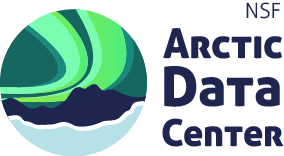
\includegraphics[width=0.49\linewidth]{images/adc_logo}

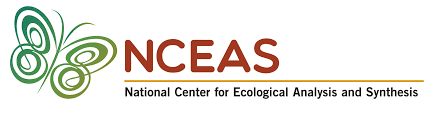
\includegraphics[width=0.49\linewidth]{images/nceas}

\hypertarget{land-acknowledgement}{%
\section*{Land Acknowledgement}\label{land-acknowledgement}}
\addcontentsline{toc}{section}{Land Acknowledgement}

This book was created on unceded Chumash ancestral lands in gratitude and solidarity with all our relations. We are committed to learning about how to implement Indigenous Data Sovereignty within our own institutions and in the trainings that Arctic Data Centers offers the Arctic research community.

The Chumash people are comprised of the descendants of Indigenous peoples removed from their Island of origin \href{https://external.as.ucsb.edu/land-acknowledgment/}{Limuw (Santa Cruz), Anyapac (Anacapa), Wima (Santa Rosa) and Tuqan (San Miguel)} subjugated by 5 missions during Spanish colonization of the Central Coast. Chumash Territory stretches from Malibu to Morro Bay and inland to Bakersfield, encompassing \href{https://www.santaynezchumash.org/chumash-history}{7,000 square miles}. The Villages, upon which University of California Santa Barbara sits, were a traditional place of knowledge sharing, education, trading and abundance.

\begin{figure}
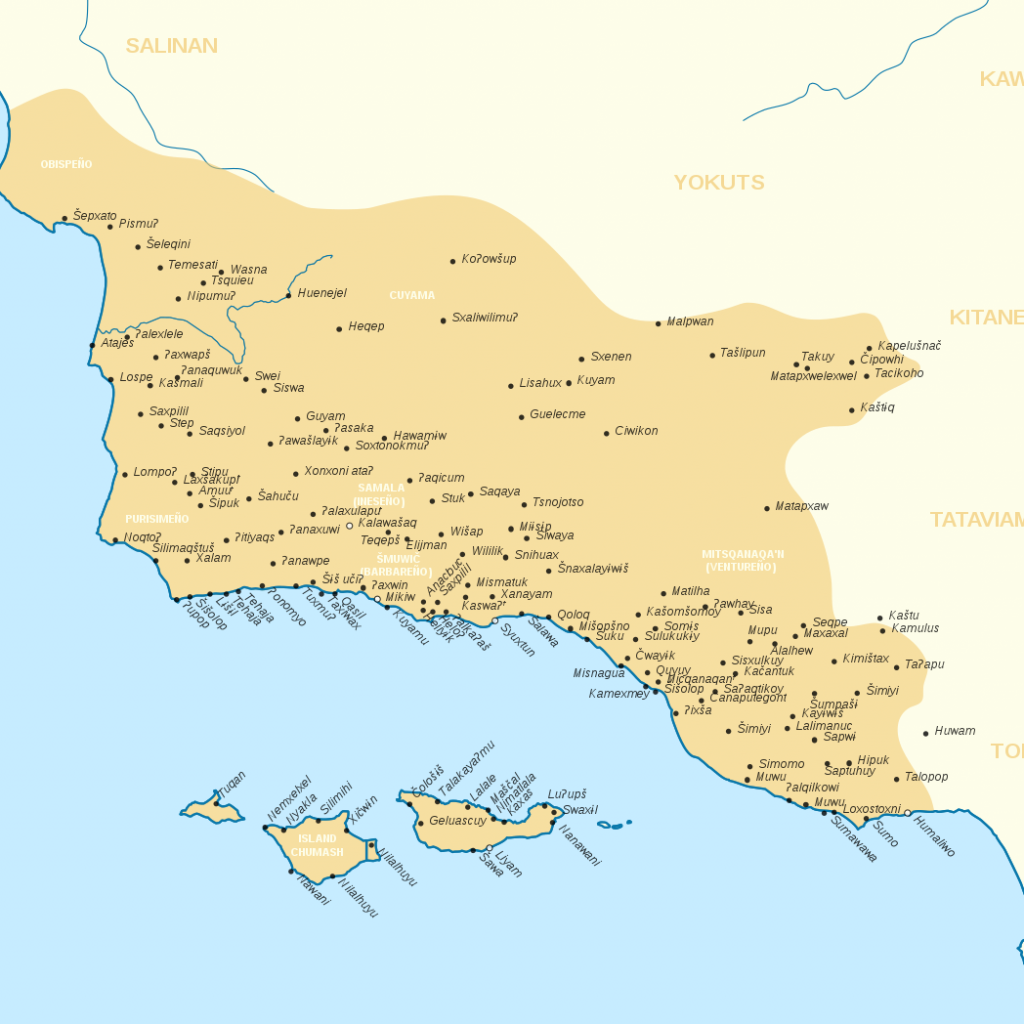
\includegraphics[width=14.22in]{images/chumash_territory} \caption{Map of Chumash Villages [source: Wikipedia Commons](https://commons.wikimedia.org/wiki/File:Chumash_villages.svg)}(\#fig:unnamed-chunk-3)
\end{figure}

If you are interested in learning more about the Chumash and how to support them, please visit their website \href{https://www.wishtoyo.org/}{here}.

\hypertarget{ids-indigenous-data-sovereignty-frameworks-networks}{%
\chapter{IDS (Indigenous Data Sovereignty) Frameworks \& Networks}\label{ids-indigenous-data-sovereignty-frameworks-networks}}

International and nation-state networks of practitioners and researchers have formed to share and develop resources and training on data management. These networks are critical for furthering Indigenous data, data sovereignty, and creating a community of Indigenous scholars and stewards.

\hypertarget{overview-of-indigenous-data-sovereignty-networks}{%
\section*{Overview of Indigenous data sovereignty networks}\label{overview-of-indigenous-data-sovereignty-networks}}
\addcontentsline{toc}{section}{Overview of Indigenous data sovereignty networks}

\begin{itemize}
\tightlist
\item
  International Groups

  \begin{itemize}
  \tightlist
  \item
    The Global Indigenous Data Alliance \href{https://www.gida-global.org/}{GIDA}
  \item
    International Indigenous Data Sovereignty Interest Group: Research Data Alliance (\href{https://www.rd-alliance.org/groups/international-indigenous-data-sovereignty-ig}{RDA})
  \end{itemize}
\item
  Anglo-settler state data sovereignty networks

  \begin{itemize}
  \tightlist
  \item
    \href{https://usindigenousdata.org/}{U.S. Indigenous Data Sovereignty Network}
  \item
    \href{https://www.temanararaunga.maori.nz/}{Te Mana Raraunga} -- Māori Data Sovereignty Network
  \item
    \href{https://www.maiamnayriwingara.org/}{The Maiam nayri Wingara Indigneous Data Sovereignty Collective}
  \end{itemize}
\end{itemize}

\hypertarget{the-global-indigenous-data-alliance-gida}{%
\subsubsection*{\texorpdfstring{The Global Indigenous Data Alliance (\href{https://www.gida-global.org/}{GIDA})}{The Global Indigenous Data Alliance (GIDA)}}\label{the-global-indigenous-data-alliance-gida}}
\addcontentsline{toc}{subsubsection}{The Global Indigenous Data Alliance (\href{https://www.gida-global.org/}{GIDA})}

Shares frameworks, tools, and processes to help guide the practice of Indigenous Data Sovereignty around the globe.
Notably, GIDA created the \href{https://www.gida-global.org/care}{CARE principles} for Indigenous Data Governance (see section 3.3).

\begin{figure}
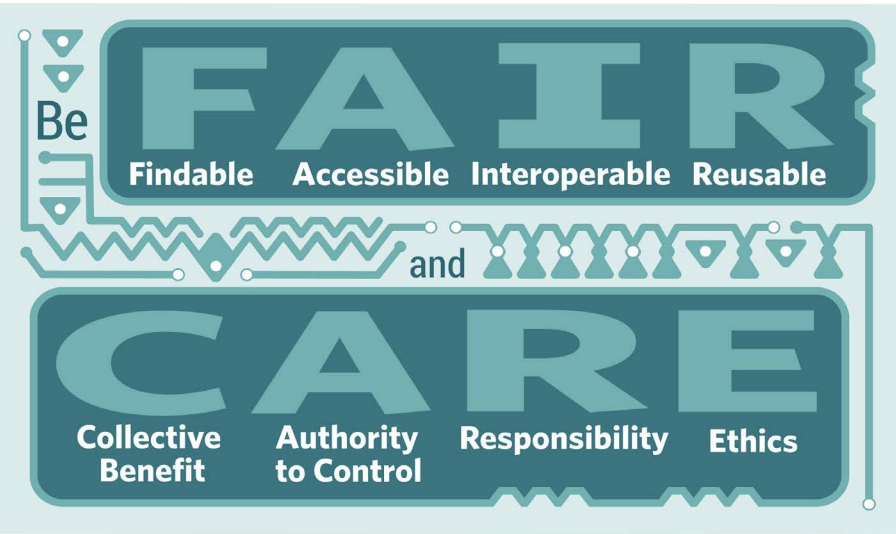
\includegraphics[width=12.44in]{images/care_fair} \caption{The CARE and FAIR Principals (GIDA 2019).}(\#fig:unnamed-chunk-4)
\end{figure}

\hypertarget{research-data-alliance-rda-international-indigenous-data-sovereignty-interest-group}{%
\subsubsection*{\texorpdfstring{Research Data Alliance (\href{https://www.rd-alliance.org/groups/international-indigenous-data-sovereignty-ig}{RDA}): International Indigenous Data Sovereignty Interest Group}{Research Data Alliance (RDA): International Indigenous Data Sovereignty Interest Group}}\label{research-data-alliance-rda-international-indigenous-data-sovereignty-interest-group}}
\addcontentsline{toc}{subsubsection}{Research Data Alliance (\href{https://www.rd-alliance.org/groups/international-indigenous-data-sovereignty-ig}{RDA}): International Indigenous Data Sovereignty Interest Group}

Builds the social and technical bridges to enable open sharing and re-use of data

\hypertarget{indigenous-statistics-the-importance-of-data-to-indigenous-communities}{%
\chapter{Indigenous Statistics: The Importance of Data to Indigenous Communities}\label{indigenous-statistics-the-importance-of-data-to-indigenous-communities}}

Indigenous peoples continue to suffer data inequities and data exploitation. Big data and secondary data are important tools for Indigenous peoples to make decisions, spur innovation and discovery, and to commercialize (\href{https://repository.oceanbestpractices.org/bitstream/handle/11329/1507/1158-8528-2-PB.pdf?sequence=1\&isAllowed=y}{Carroll et al.~2020}). While quantitative methods have long been tools of colonization, they are being rethought through an Indigenous lens. Below is a small collection of resources that discuss or present the importance of Indigenous statistics, Indigenous data and Indigenous quantitative methods.

\hypertarget{indigenous-statistics-a-quantitative-research-methodology}{%
\subsubsection{\texorpdfstring{\href{https://www.taylorfrancis.com/books/mono/10.4324/9781315426570/indigenous-statistics-maggie-walter-chris-andersen}{Indigenous statistics: A quantitative research methodology}}{Indigenous statistics: A quantitative research methodology}}\label{indigenous-statistics-a-quantitative-research-methodology}}

Maggie Walter and Chris Andersen. \emph{Routledge}, 2016.

Quantitative data on Indigenous peoples have been taken for granted as straightforward, transparent numbers. With a focus on population statistics and examples from Indigenous peoples in the United States, Australia, and Canada, Maggie Walter and Chris Anderson suggest a paradigm for Indigenous quantitative methods. This book is especially useful in understanding the systemic nature of data inequality in the context of Indigenous communities, why data is important, and how we might improve upon these systems.

\hypertarget{a-review-of-indigenous-statistics-a-quantitative-research-methodology}{%
\paragraph*{A review of Indigenous Statistics: A Quantitative Research Methodology}\label{a-review-of-indigenous-statistics-a-quantitative-research-methodology}}
\addcontentsline{toc}{paragraph}{A review of Indigenous Statistics: A Quantitative Research Methodology}

Elaine Coburn. \emph{Decolonization: Indigeneity, Education \& Society} 4.2 2015.

In this review of the book \emph{Indigenous Statistics}, Elaine Coburn makes several observations about Indigenous quantitative methodologies, focusing on the its subversion of mainstream, colonial methodologies. For example, they write: ``an important task of Indigenous quantitative methodologies is to restore visibility to colonial and Indigenous social realities that are denied by colonial statistics. As I will explore briefly below, Walter and Andersen (pp.~78-79; p.~96) suggest that this means reversing the gaze, so that the Indigenous scholar becomes the expert knower, while colonizers and non-Indigenous peoples become the ``known'' subjects of the Indigenous gaze.'' (pg. 126)

\hypertarget{indigenous-data-indigenous-methodologies-and-indigenous-data-sovereignty}{%
\subsubsection*{\texorpdfstring{\href{https://www.tandfonline.com/doi/full/10.1080/13645579.2018.1531228}{Indigenous data, indigenous methodologies and indigenous data sovereignty}}{Indigenous data, indigenous methodologies and indigenous data sovereignty}}\label{indigenous-data-indigenous-methodologies-and-indigenous-data-sovereignty}}
\addcontentsline{toc}{subsubsection}{\href{https://www.tandfonline.com/doi/full/10.1080/13645579.2018.1531228}{Indigenous data, indigenous methodologies and indigenous data sovereignty}}

Maggie Walter and Michele Suina. \emph{International Journal of Social Research Methodology} 22.3: 233-243. 2019.

Indigenous data production and collection has historically excluded Indigenous participation. Indigenous data has also been primarily analyzed qualitatively, and this paper suggests that the absence of quantitative methods that align with Indigenous methodologies has impacted statistical narratives about Indigenous Peoples. This paper explores the consequences of this absence, and focuses on Indigenous quantitative methods from a case study in New Mexico.

\hypertarget{census-powwow}{%
\subsubsection*{\texorpdfstring{\href{https://open.spotify.com/episode/28040mhUkpvUtas8bd6rmE?si=e0j9BvQ5R9m3e0AGbZajSw}{Census Powwow}}{Census Powwow}}\label{census-powwow}}
\addcontentsline{toc}{subsubsection}{\href{https://open.spotify.com/episode/28040mhUkpvUtas8bd6rmE?si=e0j9BvQ5R9m3e0AGbZajSw}{Census Powwow}}

Julian Noisecat. \emph{Snap Judgment}. June, 2021.

Journalist Julian Noisecat follows Cheyanne Brady, a member of the Mandan Hidatsa Arikara Nation, as she works to count everyone on her reservation for the US 2020 Census. This podcast details the complicated relationship tribal nations have with the US Census. Through storytelling, the listener can get a sense of the important role data has in shaping indigenous outcomes.

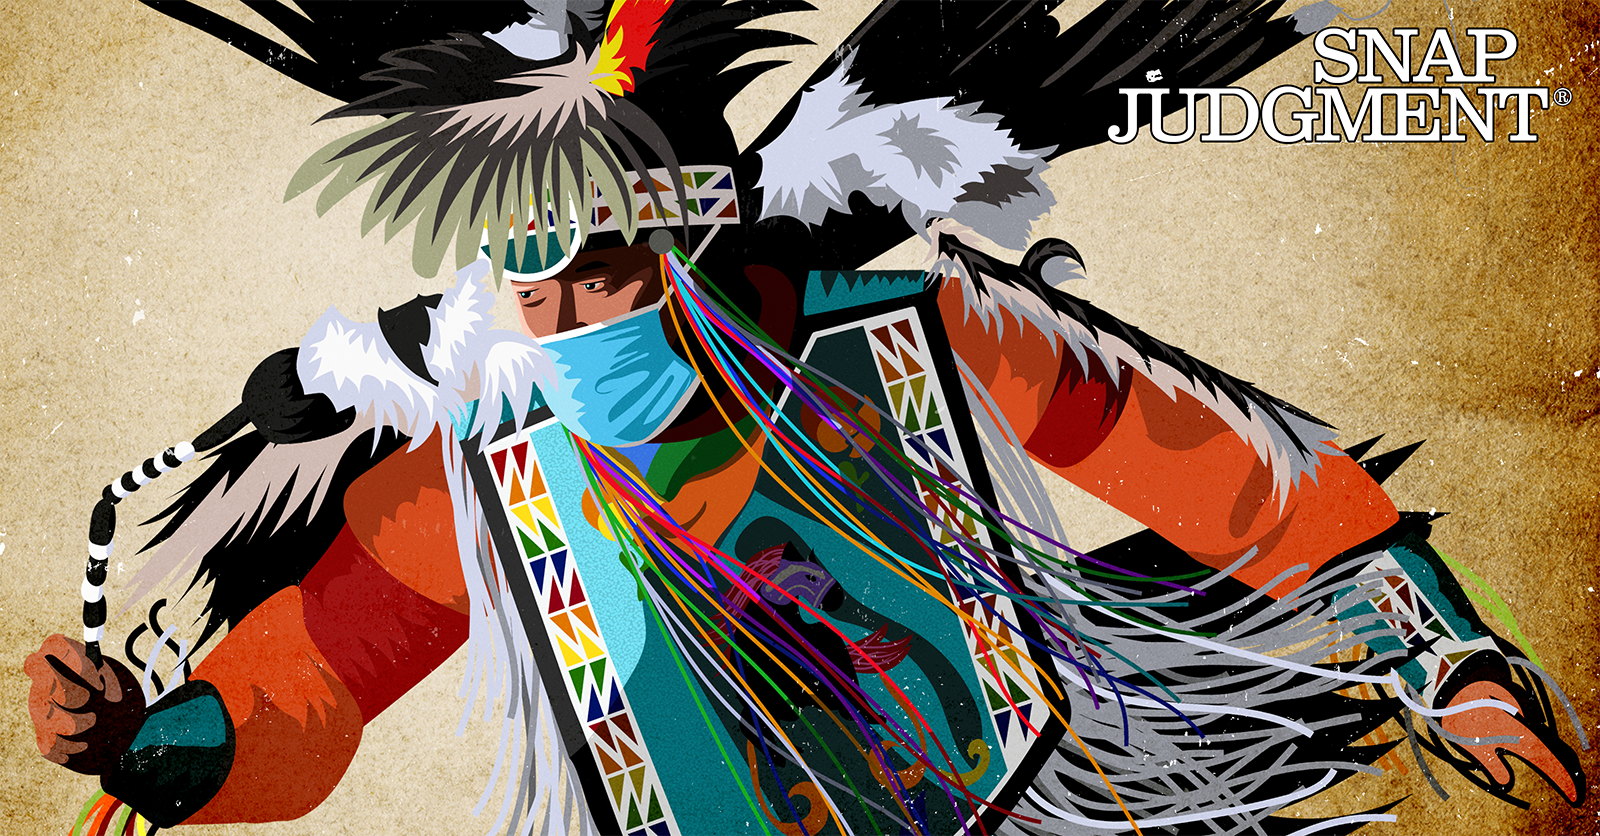
\includegraphics[width=22.22in]{images/CensusPowwow}

\hypertarget{addressing-the-need-for-indigenous-and-decolonized-quantitative-research-methods-in-canada}{%
\subsubsection*{\texorpdfstring{\href{https://www.sciencedirect.com/science/article/pii/S2352827321001749}{Addressing the need for indigenous and decolonized quantitative research methods in Canada}}{Addressing the need for indigenous and decolonized quantitative research methods in Canada}}\label{addressing-the-need-for-indigenous-and-decolonized-quantitative-research-methods-in-canada}}
\addcontentsline{toc}{subsubsection}{\href{https://www.sciencedirect.com/science/article/pii/S2352827321001749}{Addressing the need for indigenous and decolonized quantitative research methods in Canada}}

Ashley Hayward et al.~\emph{SSM-Population Health} 15: 100899. 2021.

Abstract: ``Though qualitative methods are often an appropriate Indigenous methodology and have dominated the literature on Indigenous research methods, they are not the only methods available for health research. There is a need for decolonizing and Indigenizing quantitative research methods, particularly in the discipline of epidemiology, to better address the public health needs of Indigenous populations who continue to face health inequities because of colonial systems, as well as inaccurate and incomplete data collection about themselves. For the last two decades, researchers in colonized countries have been calling for a specifically Indigenous approach to epidemiology that recognizes the limits of Western epidemiological methods, incorporates more Indigenous research methodologies and community-based participatory research methods, builds capacity by training more Indigenous epidemiologists, and supports Indigenous self-determination. Indigenous epidemiology can include a variety of approaches, including: shifting standards, such as age standardization, according to Indigenous populations to give appropriate weight to their experiences; carefully setting recruitment targets and using appropriate recruitment methods to fulfill statistical standards for stratification; acting as a bridge between Indigenous and Western technoscientific perspectives; developing culturally appropriate data collection tools; and developing distinct epidemiological methods based on Indigenous knowledge systems. This paper explores how decolonization and Indigenization of epidemiology has been operationalized in recent Canadian studies and projects, including the First Nations Regional Longitudinal Health Survey and how this decolonization and Indigenization might be augmented with the capacity-building of the future Our Health Counts Applied Indigenous Epidemiology, Health Information, and Health Services and Program Evaluation Training and Mentorship Program in Canada.''

\hypertarget{data-sovereignty-and-governance}{%
\chapter{Data Sovereignty and Governance}\label{data-sovereignty-and-governance}}

Data collection, analysis and sharing is couched in historic inequities, some of which Open Data can exacerbate. Data Sovereignty addresses aspects of data inequality, and may place limits on what data can be shared and by whom.

\textbf{Data sovereignty}: The right of a community and/or nation to maintain that data is managed in a way that is consistent with the laws, practices and customs of that community (\href{https://static1.squarespace.com/static/5d2633cb0ef5e4000134fa02/t/5d7a7610da91c0143184a9d1/1568306712324/Indigenous\%2BData\%2BSovereignty\%2BBook.pdf}{Snipp 2016}, pg. 39).

\textbf{Data governance}: ``the power to decide how and when Indigenous data are gathered, analysed, accessed and used'' (Walter et al.~2018, p.~3).

For background on these terms see \href{https://datascience.codata.org/articles/10.5334/dsj-2019-031/}{Carroll, Rodriguez-Lonebear, and Martinez 2019}.

\hypertarget{data-sovereignty}{%
\section{Data Sovereignty}\label{data-sovereignty}}

\hypertarget{indigenous-data-sovereignty-toward-an-agenda}{%
\subsubsection*{\texorpdfstring{\href{https://static1.squarespace.com/static/5d2633cb0ef5e4000134fa02/t/5d7a7610da91c0143184a9d1/1568306712324/Indigenous\%2BData\%2BSovereignty\%2BBook.pdf}{Indigenous Data Sovereignty}: Toward an Agenda}{Indigenous Data Sovereignty: Toward an Agenda}}\label{indigenous-data-sovereignty-toward-an-agenda}}
\addcontentsline{toc}{subsubsection}{\href{https://static1.squarespace.com/static/5d2633cb0ef5e4000134fa02/t/5d7a7610da91c0143184a9d1/1568306712324/Indigenous\%2BData\%2BSovereignty\%2BBook.pdf}{Indigenous Data Sovereignty}: Toward an Agenda}

Tahu Kukutai and John Taylor. \emph{ANU Press}, 2016.

\emph{Indigenous Data Sovereignty} is a book published in 2016 and is a collaboration between Indigenous scholars from Anglo-Settler states (CANSUZ), Australia, Aotearoa, the U.S. and Canada. There are 16 chapters, in which each can stand alone.

\hypertarget{indigenous-data-sovereignty-how-researchers-can-empower-data-governance}{%
\subsubsection*{\texorpdfstring{\href{https://www.youtube.com/watch?v=RjolET69Z8c}{Indigenous Data Sovereignty}: How Researchers can Empower Data Governance}{Indigenous Data Sovereignty: How Researchers can Empower Data Governance}}\label{indigenous-data-sovereignty-how-researchers-can-empower-data-governance}}
\addcontentsline{toc}{subsubsection}{\href{https://www.youtube.com/watch?v=RjolET69Z8c}{Indigenous Data Sovereignty}: How Researchers can Empower Data Governance}

Lydia Jennings. \emph{NCEAS Seminar Series}. 2021.

In a NCEAS seminar, Lydia Jennings (Postdoc UofA, Collaboratory for Indigenous Data Governance), provides an overview of Indigenous Data Sovereignty, especially as it pertains to environmental science.

\hypertarget{being-in-good-community-engagement-in-support-of-indigenous-sovereignty}{%
\subsubsection*{\texorpdfstring{``\href{https://www.tandfonline.com/doi/full/10.1080/15265161.2021.1965243}{Being in Good Community: Engagement in Support of Indigenous Sovereignty}''}{``Being in Good Community: Engagement in Support of Indigenous Sovereignty''}}\label{being-in-good-community-engagement-in-support-of-indigenous-sovereignty}}
\addcontentsline{toc}{subsubsection}{``\href{https://www.tandfonline.com/doi/full/10.1080/15265161.2021.1965243}{Being in Good Community: Engagement in Support of Indigenous Sovereignty}''}

Jessica Blanchard and Vanessa Hiratsuka. \emph{The American Journal of Bioethics} 21.10. 54-56. 2021.

Blanchard and Hiratsuka, researchers at The Center for the Ethics of Indigenous Genomic Research (CEIGR), advocate for the assertion of tribal sovereignty as a guiding principle for more ethical, community-engaged research with tribes.

\hypertarget{indigenous-data-sovereignty}{%
\subsubsection*{\texorpdfstring{``\href{https://open.spotify.com/episode/3T7XBXU28bghKTPlowEuHL?si=SbeZZ12FQrSC0zbNkt4REA\&nd=1}{Indigenous data sovereignty}''}{``Indigenous data sovereignty''}}\label{indigenous-data-sovereignty}}
\addcontentsline{toc}{subsubsection}{``\href{https://open.spotify.com/episode/3T7XBXU28bghKTPlowEuHL?si=SbeZZ12FQrSC0zbNkt4REA\&nd=1}{Indigenous data sovereignty}''}

\emph{IndigenousX Presents: Blak Nation}. August 31, 2021.

Blak Nation's ``Indigenous data sovereignty'' is a podcast episode that interviews Dr.~Maggie Walter, co-author of Indigenous Statistics, Dr.~Maui Hudson (Professor and Director or Te Kotahi Research Institute), Dr.~Jane Anderson (Professor at NYU and co-founder of Local Contexts), and Dr.~Kalinda Griffiths (Scientia Lecturer at Centre for Big Data Research in Health, UNSW Sydney). Dr.~Walter opens the podcast with an overview of the Indigenous Data Sovereignty movement, while Hudson, Anderson and Griffiths provide specific examples.

\hypertarget{indigenous-data-sovereignty-in-the-era-of-big-data-and-open-data}{%
\subsubsection*{\texorpdfstring{``\href{https://onlinelibrary.wiley.com/doi/full/10.1002/ajs4.141}{Indigenous data sovereignty in the era of big data and open data}''}{``Indigenous data sovereignty in the era of big data and open data''}}\label{indigenous-data-sovereignty-in-the-era-of-big-data-and-open-data}}
\addcontentsline{toc}{subsubsection}{``\href{https://onlinelibrary.wiley.com/doi/full/10.1002/ajs4.141}{Indigenous data sovereignty in the era of big data and open data}''}

Maggie Walter et al.~\emph{Australian Journal of Social Issues} 56.2: 143-156. 2021.

Abstract: ``Indigenous Data Sovereignty, in its proclamation of the right of Indigenous peoples to govern the collection, ownership, and application of data, recognises data as a cultural and economic asset. The impact of data is magnified by the emergence of Big Data and the associated impetus to open publicly held data (Open Data). Aboriginal and Torres Strait Islander peoples, families and communities, heavily overrepresented in social disadvantage--related data will also be overrepresented in the application of these new technologies, but in a data landscape, Indigenous peoples remain largely alienated from the use of data and its utilization within the channels of policy power. Existing data infrastructure, and the emerging Open Data infrastructure, neither recognise Indigenous agency and worldviews nor consider Indigenous data needs. This is demonstrated in the absence of any consideration of Indigenous data issues in Open Data discussions and publication. Thus, while the potential benefits of this data revolution are trumpeted, our marginalised social, cultural and political location suggests we will not share equally in these benefits. This paper discusses the unforeseen (and likely unseen) consequences of the influence of Open Data and Big Data and discusses how Indigenous Data Sovereignty can mediate risks while providing pathways to collective benefits.''

\hypertarget{data-governance}{%
\section{Data Governance}\label{data-governance}}

\hypertarget{indigenous-data-governance-strategies-from-united-states-native-nations}{%
\subsubsection*{\texorpdfstring{``\href{https://datascience.codata.org/articles/10.5334/dsj-2019-031/}{Indigenous Data Governance}: Strategies from United States Native Nations''}{``Indigenous Data Governance: Strategies from United States Native Nations''}}\label{indigenous-data-governance-strategies-from-united-states-native-nations}}
\addcontentsline{toc}{subsubsection}{``\href{https://datascience.codata.org/articles/10.5334/dsj-2019-031/}{Indigenous Data Governance}: Strategies from United States Native Nations''}

Stephanie Russo Carroll, Desi Rodriguez-Lonebear, and Andrew Martinez. \emph{Data Science Journal}, 18(1), p.31. 2019.

This review paper argues for the repositioning of authority over Indigenous data back to Indigenous peoples through context setting and case studies. For those wanting an overview to these concepts, Carroll, Rodriguez-Lonebear and Martinez provide an especially background of key terms related to data sovereignty and data governance.

\begin{figure}
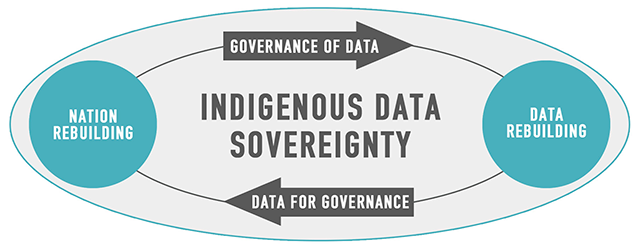
\includegraphics[width=8.89in]{images/download} \caption{Building Indigenous data soverigenty through Indigenous data governance}(\#fig:unnamed-chunk-6)
\end{figure}

\hypertarget{the-voice-of-indigenous-data-beyond-the-markers-of-disadvantage}{%
\subsubsection*{\texorpdfstring{``\href{https://www.griffithreview.com/articles/voice-indigenous-data-beyond-disadvantage/}{The voice of indigenous data: beyond the markers of disadvantage}''}{``The voice of indigenous data: beyond the markers of disadvantage''}}\label{the-voice-of-indigenous-data-beyond-the-markers-of-disadvantage}}
\addcontentsline{toc}{subsubsection}{``\href{https://www.griffithreview.com/articles/voice-indigenous-data-beyond-disadvantage/}{The voice of indigenous data: beyond the markers of disadvantage}''}

Maggie Walter. \emph{Griffith Review} 60: 256-263. 2018.

Maggie Walter outlines the Indigenous Data Paradox: there is both too much data about Aboriginal and Torres Strait Islander people but almost no data for or by Aboriginal and Torres Strait Islander people. Walter then maps these data failures across data categories, ultimately calling for a change in the paradigm of Indigenous data.

\hypertarget{first-nations-data-sovereignty}{%
\subsubsection*{\texorpdfstring{``\href{https://open.spotify.com/episode/7lpJvcWPEX0DJcMjQPTdiK?si=r3AfZ-SbQeu3KrMtPbK6cQ}{First Nations data sovereignty}''}{``First Nations data sovereignty''}}\label{first-nations-data-sovereignty}}
\addcontentsline{toc}{subsubsection}{``\href{https://open.spotify.com/episode/7lpJvcWPEX0DJcMjQPTdiK?si=r3AfZ-SbQeu3KrMtPbK6cQ}{First Nations data sovereignty}''}

\emph{Info Matters}. August 2021.

Info Matters is a podcast by the Information and Privacy Commissioner of Ontario, Canada, Patricia Kosseim. In this episode, Kosseim interviews Dr.~Jonathan Dewer, Chief Executive Officer of the First Nations Information Governance Center, and Carmen Jones, Director of Research and Data Management for the Chief of Ontario. Dewar and Jones provide unique insight into data sovereignty broadly and specifically the creation and implementation of OCAP Principals (14:15).

\hypertarget{good-data-practices-for-indigenous-data-sovereignty-and-governance}{%
\subsubsection*{\texorpdfstring{``\href{https://books.google.com/books?hl=en\&lr=\&id=Y0vUDwAAQBAJ\&oi=fnd\&pg=PA26\&dq=Good+data+practices+for+Indigenous+data+sovereignty+and+governance\&ots=hr9XhjlbCh\&sig=QKNc1PnCBYMO2s1mHYWbRg6g_GU\#v=onepage\&q=Good\%20data\%20practices\%20for\%20Indigenous\%20data\%20sovereignty\%20and\%20governance\&f=false}{Good data practices for Indigenous data sovereignty and governance}''}{``Good data practices for Indigenous data sovereignty and governance''}}\label{good-data-practices-for-indigenous-data-sovereignty-and-governance}}
\addcontentsline{toc}{subsubsection}{``\href{https://books.google.com/books?hl=en\&lr=\&id=Y0vUDwAAQBAJ\&oi=fnd\&pg=PA26\&dq=Good+data+practices+for+Indigenous+data+sovereignty+and+governance\&ots=hr9XhjlbCh\&sig=QKNc1PnCBYMO2s1mHYWbRg6g_GU\#v=onepage\&q=Good\%20data\%20practices\%20for\%20Indigenous\%20data\%20sovereignty\%20and\%20governance\&f=false}{Good data practices for Indigenous data sovereignty and governance}''}

Raymond Lovett et al.~\emph{Good Data}: 26-36. 2019.

``This chapter aims to provide clarity concerning the definitions of Indigenous Data Sovereignty (IDS) and Indigenous Data Governance (IDG); provide an overview of the historical context in which IDS has emerged; and provide examples of IDS and IDG across the spectrum of community, policy, and practice.''

\hypertarget{guidelines-for-and-for-working-with-indigenous-nations}{%
\section{Guidelines for and for Working With Indigenous Nations}\label{guidelines-for-and-for-working-with-indigenous-nations}}

\hypertarget{the-care-principles-for-indigenous-data-governance}{%
\subsection{The CARE Principles for Indigenous Data Governance}\label{the-care-principles-for-indigenous-data-governance}}

\hypertarget{the-care-principles-for-indigenous-data-governance-1}{%
\subsubsection*{\texorpdfstring{``\href{http://doi.org/10.5334/dsj-2020-043}{The CARE Principles for Indigenous Data Governance}''}{``The CARE Principles for Indigenous Data Governance''}}\label{the-care-principles-for-indigenous-data-governance-1}}
\addcontentsline{toc}{subsubsection}{``\href{http://doi.org/10.5334/dsj-2020-043}{The CARE Principles for Indigenous Data Governance}''}

Carroll, Stephanie Russo, Ibrahim Garba, Oscar L. Figueroa-Rodríguez, Jarita Holbrook, Raymond Lovett, Simeon Materechera, Mark Parsons, Kay Raseroka, Desi Rodriguez-Lonebear, Robyn Rowe, Rodrigo Sara, Jennifer D. Walker, Jane Anderson, Maui Hudson. \emph{Data Science Journal}, 19(1), p.43. 2020

The `CARE Principles for Indigenous Data Governance' (Collective Benefit, Authority to Control, Responsibility, and Ethics) were developed due to concerns about secondary use of data and limited opportunities for benefit-sharing between Indigenous communities and outside researchers. While the FAIR Principles are data-centric, the CARE Principles are people and purpose oriented. The authors write, ``the goal is that stewards and other users of Indigenous data will `Be FAIR and CARE.'\,'' CARE principles are intended to be used in concert with FAIR Principals. Of particular note, this paper also provides an important background on Indigenous data sovereignty.

\begin{figure}
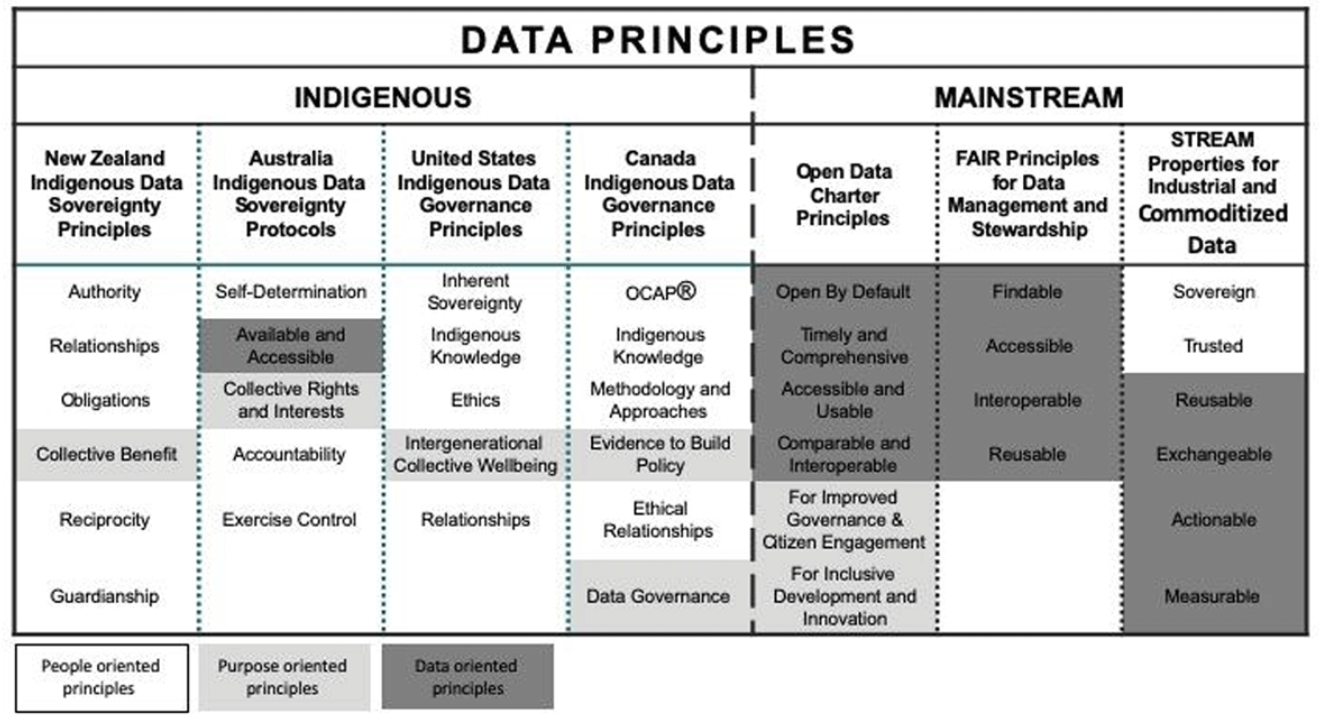
\includegraphics[width=18.39in]{images/care} \caption{Indigenous and mainstream data principles, and the orientation of these principles towards data, people and purpose (Carroll et al. 2020).}(\#fig:unnamed-chunk-7)
\end{figure}

\hypertarget{operationalizing-the-care-and-fair-principles-for-indigenous-data-futures}{%
\subsubsection*{\texorpdfstring{``\href{https://doi.org/10.1038/s41597-021-00892-0}{Operationalizing the CARE and FAIR Principles for Indigenous data futures}''}{``Operationalizing the CARE and FAIR Principles for Indigenous data futures''}}\label{operationalizing-the-care-and-fair-principles-for-indigenous-data-futures}}
\addcontentsline{toc}{subsubsection}{``\href{https://doi.org/10.1038/s41597-021-00892-0}{Operationalizing the CARE and FAIR Principles for Indigenous data futures}''}

Stephanie Russo Carroll, et al.~\emph{Scientific Data} 8, no. 1. 2021.

CARE Principles place emphasis on placing intention and human well-being at the forefront of data publishing and sharing. While FAIR principles are often used in the context of open science, they differ from open science, and represent guidelines for publishing data that can be easily interpreted, stand the test of time, and reused if applicable. Together, CARE and FAIR principles speak to clean, well-managed data that puts human well-being first.

\hypertarget{using-indigenous-standards-to-implement-the-care-principles-setting-expectations-through-tribal-research-codes}{%
\subsubsection*{\texorpdfstring{``\href{https://www.frontiersin.org/articles/10.3389/fgene.2022.823309/full?\&utm_source=Email_to_authors_\&utm_medium=Email\&utm_content=T1_11.5e1_author\&utm_campaign=Email_publication\&field=\&journalName=Frontiers_in_Genetics\&id=823309}{Using Indigenous Standards to Implement the CARE Principles: Setting Expectations through Tribal Research Codes}''}{``Using Indigenous Standards to Implement the CARE Principles: Setting Expectations through Tribal Research Codes''}}\label{using-indigenous-standards-to-implement-the-care-principles-setting-expectations-through-tribal-research-codes}}
\addcontentsline{toc}{subsubsection}{``\href{https://www.frontiersin.org/articles/10.3389/fgene.2022.823309/full?\&utm_source=Email_to_authors_\&utm_medium=Email\&utm_content=T1_11.5e1_author\&utm_campaign=Email_publication\&field=\&journalName=Frontiers_in_Genetics\&id=823309}{Using Indigenous Standards to Implement the CARE Principles: Setting Expectations through Tribal Research Codes}''}

Stephanie Russo Carroll, et al.~\emph{Frontiers in Genetics} 489. 2022.

Abstract Excerpt: ``This article outlines the relationship between sovereignty and ethics in the context of data to describe the collective rights that Indigenous Peoples assert to increase control over their biomedical data. Then drawing on the CARE Principles for Indigenous Data Governance (Collective benefit, Authority to control, Responsibility, and Ethics), we explore how standards already set by Native nations in the United States, such as tribal research codes, provide direction for implementation of the CARE Principles to complement FAIR. A broader approach to policy and procedure regarding tribal participation in biomedical research is required and we make recommendations for tribes, institutions, and ethical practice.''

\hypertarget{ocap-principals}{%
\subsection{OCAP Principals}\label{ocap-principals}}

\hypertarget{ocap---first-nations-ownership-control-access-and-possession-or-self-determination-applied-to-research-2004}{%
\subsubsection*{\texorpdfstring{\href{https://biblio.uottawa.ca/sites/biblio.uottawa.ca/files/bestpractices_fnigc_ocap_fact_sheet_en_final.pdf}{OCAP - First Nations Ownership, Control, Access and Possession or Self Determination Applied to Research (2004)}}{OCAP - First Nations Ownership, Control, Access and Possession or Self Determination Applied to Research (2004)}}\label{ocap---first-nations-ownership-control-access-and-possession-or-self-determination-applied-to-research-2004}}
\addcontentsline{toc}{subsubsection}{\href{https://biblio.uottawa.ca/sites/biblio.uottawa.ca/files/bestpractices_fnigc_ocap_fact_sheet_en_final.pdf}{OCAP - First Nations Ownership, Control, Access and Possession or Self Determination Applied to Research (2004)}}

The OCAP Principals were first developed in 1998 in response to extractive research practices. ``These principals establish how First Nations' data, information, and cultural knowledge should be collected, accessed, used, and shared.''

\hypertarget{fundamentals-of-ocap-course}{%
\subsubsection*{\texorpdfstring{\href{https://fnigc.ca/ocap-training/take-the-course/}{Fundamentals of OCAP Course}}{Fundamentals of OCAP Course}}\label{fundamentals-of-ocap-course}}
\addcontentsline{toc}{subsubsection}{\href{https://fnigc.ca/ocap-training/take-the-course/}{Fundamentals of OCAP Course}}

An online training course to introduce individuals to the fundamental concepts of OCAP, information governance, and First Nations Data Sovereignty.

\hypertarget{data-management-tools}{%
\chapter{Data Management Tools}\label{data-management-tools}}

Thus far, the data management tools we've come across have largely been developed by \href{https://localcontexts.org/labels/biocultural-labels/}{Local Contexts}. If you have examples of other practical tools or organizations that develop them, please share!

\hypertarget{biocultural-labels}{%
\section{Biocultural Labels}\label{biocultural-labels}}

Data labels are text elements that describe individual data points. They are used on metadata as a tag that can be easily categorized and searched. Biocultural (BC) labels are data-markers being piloted by the \href{https://www.enrich-hub.org/bc-labels}{The Biocultural Label Initiative} to help define community expectations and consent about research data use. ``The BC Labels provide a practical application of Indigenous data sovereignty principles to issues of access and benefit-sharing for genetic resources and support Nagoya Protocol expectations around the disclosure and origins of Indigenous data used in research contexts.'' (Anderson \& Hudson 2021)

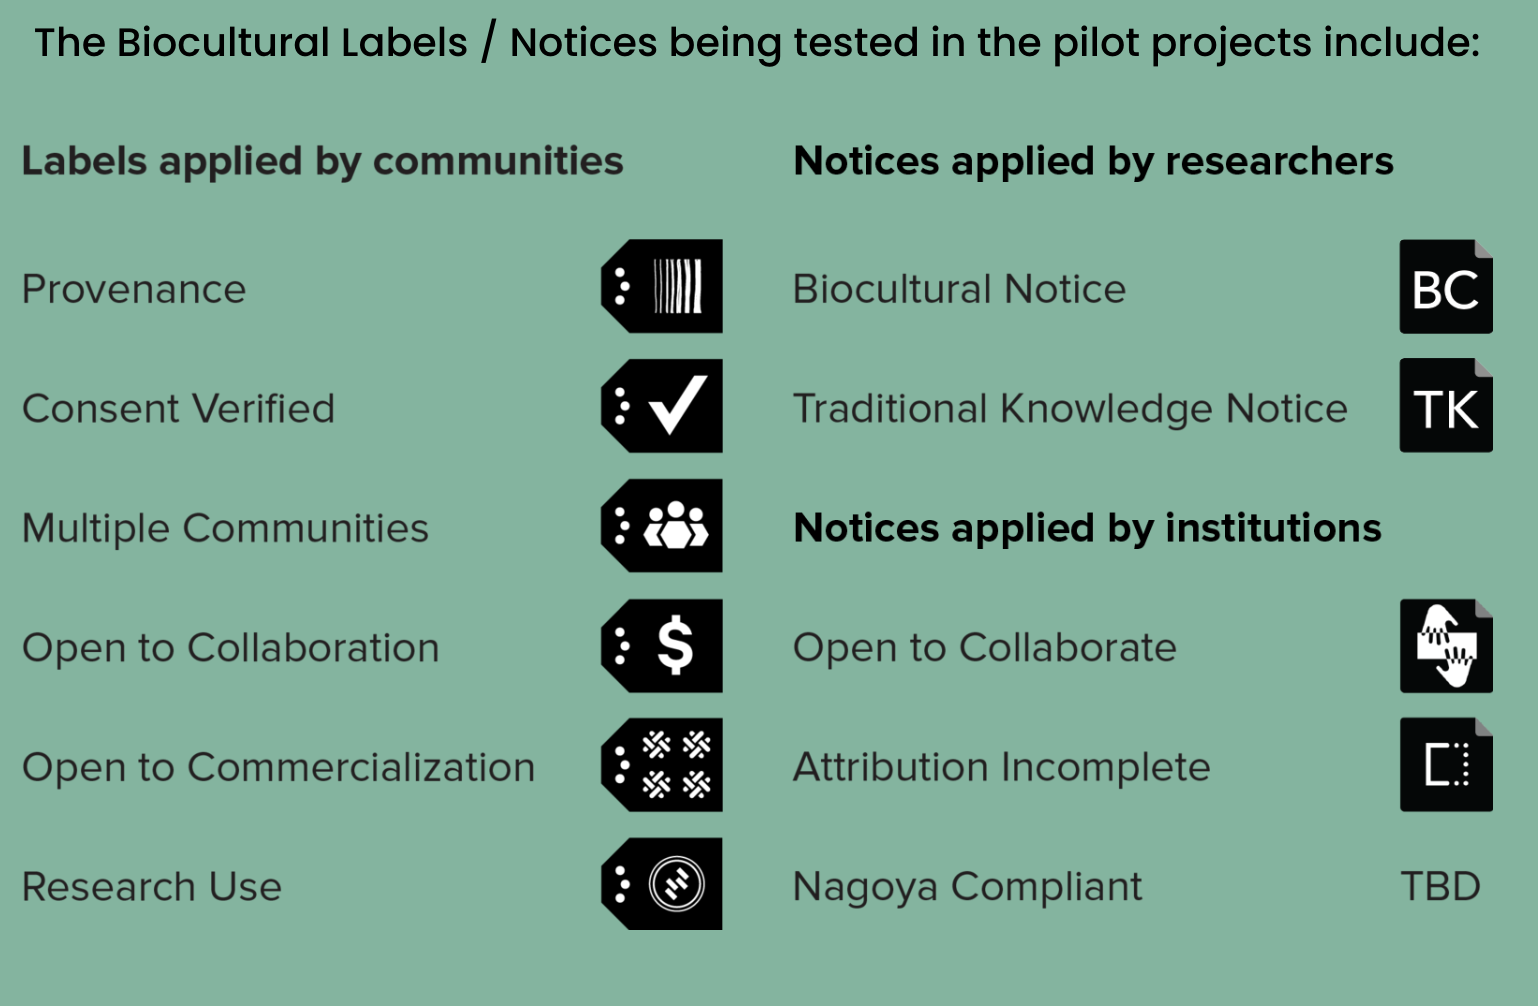
\includegraphics[width=21.36in]{images/biocultural_labels}

\hypertarget{the-biocultural-labels-initiative}{%
\subsubsection*{\texorpdfstring{\href{https://qubeshub.org/publications/2326/1}{The Biocultural Labels Initiative}}{The Biocultural Labels Initiative}}\label{the-biocultural-labels-initiative}}
\addcontentsline{toc}{subsubsection}{\href{https://qubeshub.org/publications/2326/1}{The Biocultural Labels Initiative}}

Jane Anderson and Maui Hudson. \emph{STEM Inclusive Teaching Practices Webinar Series}. 2021.

This webinar series is geared towards facilitating inclusive teaching practices with undergraduates. Here, Jane Anderson and Maui Hudson introduce Biocultural Labels and the work of Local Contexts.

\hypertarget{indigenous-digitial-strategies}{%
\section{Indigenous Digitial Strategies}\label{indigenous-digitial-strategies}}

\hypertarget{local-contexts}{%
\subsubsection*{\texorpdfstring{\href{https://localcontexts.org/labels/biocultural-labels/}{Local Contexts}}{Local Contexts}}\label{local-contexts}}
\addcontentsline{toc}{subsubsection}{\href{https://localcontexts.org/labels/biocultural-labels/}{Local Contexts}}

Local Contexts is an organization that offers digital strategies for Indigenous communities, cultural institutions and researchers through Traditional Knowledge and Biocultural Labels and Notices and licenses for intellectual property.

\hypertarget{open-data-principals}{%
\chapter{Open Data Principals}\label{open-data-principals}}

The Open Data movement has had significant success. Data is more accessible than ever before. The Findable, Accessible, Interoperable and Reusable (FAIR) Data Principles were developed to improve the reuse of scholarly data. However, data collection, analysis and sharing is couched in historic inequities. The FAIR principles, now paired with CARE, can work together to ensure data is ethically sourced and shared.

\hypertarget{fair-principals}{%
\subsection{FAIR Principals}\label{fair-principals}}

\hypertarget{the-fair-guiding-principles-for-scientific-data-management-and-stewardship}{%
\subsubsection*{\texorpdfstring{``\href{https://www.nature.com/articles/sdata201618}{The FAIR Guiding Principles for scientific data management and stewardship}''}{``The FAIR Guiding Principles for scientific data management and stewardship''}}\label{the-fair-guiding-principles-for-scientific-data-management-and-stewardship}}
\addcontentsline{toc}{subsubsection}{``\href{https://www.nature.com/articles/sdata201618}{The FAIR Guiding Principles for scientific data management and stewardship}''}

Mark D. Wilkinson, et al.~\emph{Scientific Data} 3.1: 1-9. 2016.

The Findable, Accessible, Interoperable and Reusable (FAIR) Data principles were developed in reaction to the wide reuse of scholarly data. They have become increasingly important, acting as guidelines to improve the entire lifecycle of research data management (D7.4 2021). The term ``FAIR'' was first developed at a Lorentz workshop in the Netherlands in 2014 (D7.4 2021).

\hypertarget{the-fair-guiding-principles-for-data-stewardship-fair-enough}{%
\subsubsection*{\texorpdfstring{``\href{https://www.ncbi.nlm.nih.gov/pmc/articles/PMC6018669/}{The FAIR guiding principles for data stewardship: fair enough?}''}{``The FAIR guiding principles for data stewardship: fair enough?''}}\label{the-fair-guiding-principles-for-data-stewardship-fair-enough}}
\addcontentsline{toc}{subsubsection}{``\href{https://www.ncbi.nlm.nih.gov/pmc/articles/PMC6018669/}{The FAIR guiding principles for data stewardship: fair enough?}''}

Martin Boeckhout, Gerhard A. Zielhuis, and Annelien L. Bredenoord. \emph{European Journal of Human Genetics} 26.7: 931-936. 2018.

Abstract: ``The FAIR guiding principles for research data stewardship (findability, accessibility, interoperability, and reusability) look set to become a cornerstone of research in the life sciences. A critical appraisal of these principles in light of ongoing discussions and developments about data sharing is in order. The FAIR principles point the way forward for facilitating data sharing more systematically---provided that a number of ethical, methodological, and organisational challenges are addressed as well.''

\hypertarget{d7.4-how-to-be-fair-with-your-data}{%
\subsubsection*{\texorpdfstring{D7.4 \href{https://zenodo.org/record/5837500\#.Yhk8L5PMJ6e}{How to be FAIR with your data}}{D7.4 How to be FAIR with your data}}\label{d7.4-how-to-be-fair-with-your-data}}
\addcontentsline{toc}{subsubsection}{D7.4 \href{https://zenodo.org/record/5837500\#.Yhk8L5PMJ6e}{How to be FAIR with your data}}

\emph{A teaching and training handbook for higher education institutions}. November 2021.

The handbook was written and edited by a group of about 40 collaborators as part of a working group and was subject to community review. The 179 page book is a wealth of information and practical materials relating to the FAIR principals. Practical materials include competence profiles, learning outcomes and lesson plans, and supporting information.

\hypertarget{fair-and-beyond}{%
\subsection{FAIR and Beyond}\label{fair-and-beyond}}

For CARE Principals, see Section 3.3: Guidelines for and for Working With Indigenous Nations

\hypertarget{fostering-global-data-sharing-highlighting-the-recommendations-of-the-research-data-alliance-covid-19-working-group.}{%
\subsubsection*{\texorpdfstring{``\href{https://www.ncbi.nlm.nih.gov/pmc/articles/PMC7808050/}{Fostering global data sharing: highlighting the recommendations of the Research Data Alliance COVID-19 working group.}''}{``Fostering global data sharing: highlighting the recommendations of the Research Data Alliance COVID-19 working group.''}}\label{fostering-global-data-sharing-highlighting-the-recommendations-of-the-research-data-alliance-covid-19-working-group.}}
\addcontentsline{toc}{subsubsection}{``\href{https://www.ncbi.nlm.nih.gov/pmc/articles/PMC7808050/}{Fostering global data sharing: highlighting the recommendations of the Research Data Alliance COVID-19 working group.}''}

Claire C. Austin, et al.~\emph{Wellcome Open Research} 5. 2020.

This letter, developed by a 160 person international working group, shares a set of recommendations and guidelines on data sharing and best practices for COVID-19 research. Here, the authors create recommendations that balance adherence to FAIR Principles but given the nature of COVID-19, also need quick data release.

\hypertarget{examples-of-indigenous-environmental-synthesis-and-data-science}{%
\chapter{Examples of Indigenous Environmental Synthesis and Data Science}\label{examples-of-indigenous-environmental-synthesis-and-data-science}}

\hypertarget{environmental-synthesis}{%
\section{Environmental Synthesis}\label{environmental-synthesis}}

\hypertarget{a-spatial-overview-of-the-global-importance-of-indigenous-lands-for-conservation}{%
\subsubsection*{\texorpdfstring{``\href{https://www.nature.com/articles/s41893-018-0100-6?ss_source=sscampaigns\&ss_campaign_id=5c424fe9d20e280001eb02bf\&ss_email_id=5c5cf4c39bca21000175c9fd\&ss_campaign_name=Introducing+the+Interfaith+Rainforest+Initiative\&ss_campaign_sent_date=2019-02-08T03:17:24Z}{A spatial overview of the global importance of Indigenous lands for conservation}''}{``A spatial overview of the global importance of Indigenous lands for conservation''}}\label{a-spatial-overview-of-the-global-importance-of-indigenous-lands-for-conservation}}
\addcontentsline{toc}{subsubsection}{``\href{https://www.nature.com/articles/s41893-018-0100-6?ss_source=sscampaigns\&ss_campaign_id=5c424fe9d20e280001eb02bf\&ss_email_id=5c5cf4c39bca21000175c9fd\&ss_campaign_name=Introducing+the+Interfaith+Rainforest+Initiative\&ss_campaign_sent_date=2019-02-08T03:17:24Z}{A spatial overview of the global importance of Indigenous lands for conservation}''}

Garnett, Stephen T., et al.~\emph{Nature Sustainability} 1.7: 369-374. 2018.

This paper provides the first global assessment of global lands within Indigenous stewardship and it's overlap with protected areas and conservation outcomes. The authors found that Indigenous Peoples have tenure rights or actively manage more than a quarter of the world's land surface (\textasciitilde38 million km\textsuperscript{2} across 87 countries). Indigenous managed lands account for about 40\% of all terrestrial protected areas and ecologically intact landscapes (for example, boreal and tropical primary forests, savannas and marshes). Thus, indigenous stewarded lands are critical hubs for biodiversity and resilience.

To create this global assessment, the authors rely on 127 publicly available data sources, including real estate (cadastral) records for state-recognized Indigenous Peoples' lands, publicly accessible participatory mapping, models based on census data and maps derived from scholarly publications. Here, the authors worked to overcome some of the inherent biases in Indigenous geospatial data. Data of Indigenous Peoples' land occupation or management tend to rely on state-sanctioned data that can be deployed to disenfranchise Indigenous Peoples (\href{https://www.sciencedirect.com/science/article/pii/S0016718510001090?via\%3Dihub}{Bryan 2011}; Garnett et al.~2018). The authors write, ``the dearth of reliable data on Indigenous Peoples' lands in many parts of the world has implications not only for securing their rights but also for the conservation and management of a significant proportion of terrestrial global biodiversity.''

\begin{figure}
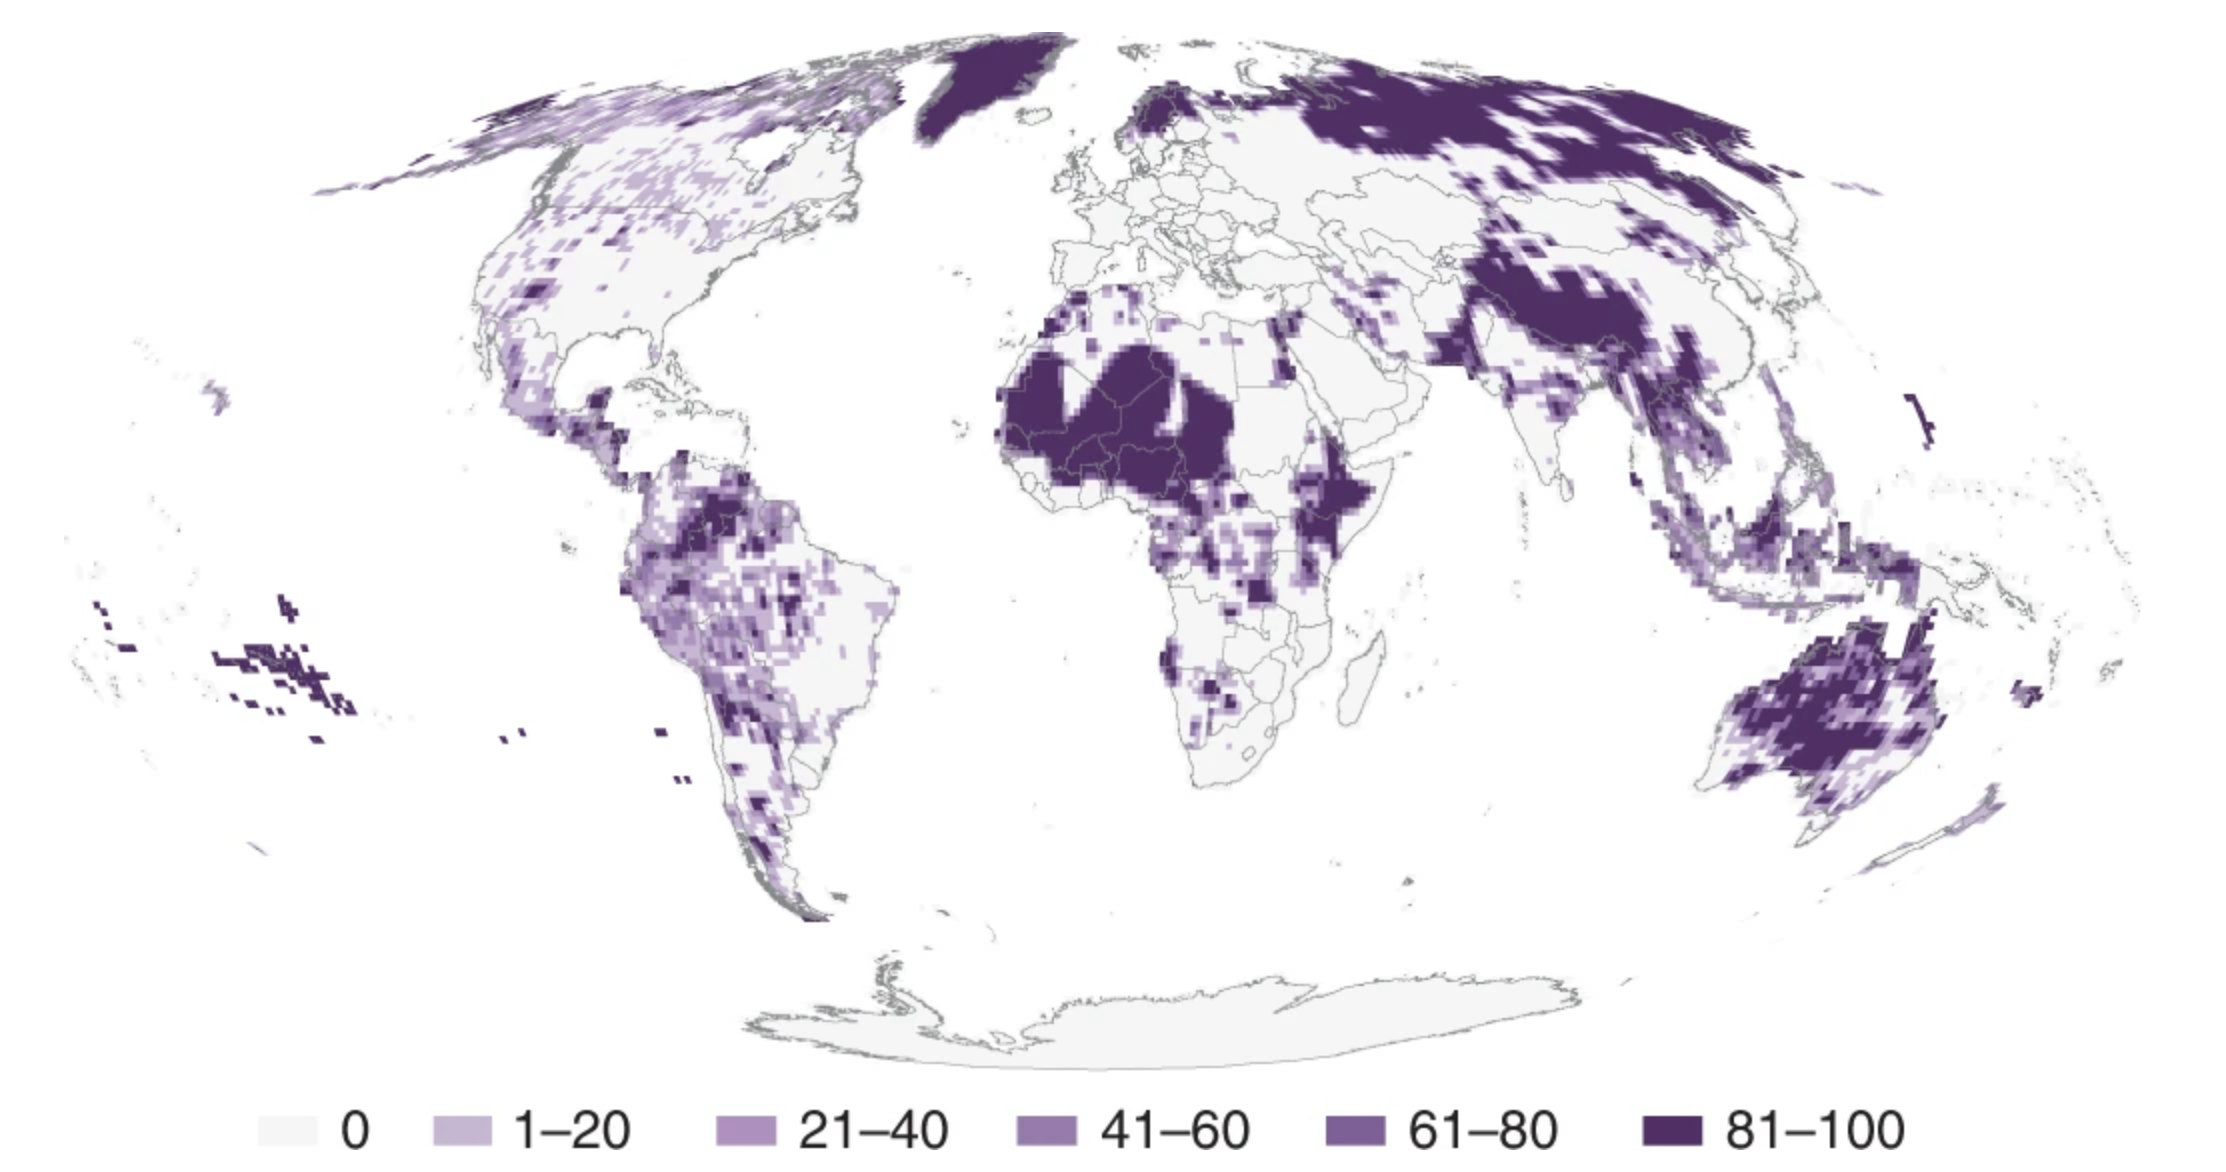
\includegraphics[width=30.92in]{images/Garnett_2018} \caption{Global map of lands managed or controlled by Indigengous Peoples. Purple shading represents the percentage of each degree square mapped as Indigenous in at least one of 127 source documents. Blank areas do not neccesarily indicate an absence of Indigenous Peoples or lands (Garnett et al. 2018).}(\#fig:unnamed-chunk-9)
\end{figure}

\hypertarget{indigenous-environmental-data}{%
\section{Indigenous Environmental Data}\label{indigenous-environmental-data}}

\hypertarget{indigenous-climate-knowledge-and-data-sovereignty}{%
\subsubsection*{\texorpdfstring{``\href{https://open.spotify.com/episode/4Gdp1RSChCPM0qftRun3DD?si=pcVeYiwwQIWnlKynt4-ADQ}{Indigenous Climate Knowledge and Data Sovereignty}''}{``Indigenous Climate Knowledge and Data Sovereignty''}}\label{indigenous-climate-knowledge-and-data-sovereignty}}
\addcontentsline{toc}{subsubsection}{``\href{https://open.spotify.com/episode/4Gdp1RSChCPM0qftRun3DD?si=pcVeYiwwQIWnlKynt4-ADQ}{Indigenous Climate Knowledge and Data Sovereignty}''}

\emph{Warm Regards}. February 2021.

Warm Regards is a podcast about life on a warming planet. In this episode, the hosts interview two Indigenous scientists, James Rattling Leaf, Sr.~and Krystal Tsosie, about traditional ecological knowledges and data sovereignty.

\hypertarget{traditional-ecological-knowledge-tek-applications-to-management}{%
\section{Traditional Ecological Knowledge (TEK) applications to management}\label{traditional-ecological-knowledge-tek-applications-to-management}}

Below are a couple examples which speak to how TEK and other forms of knowledge, such as western science, can work together to increase understanding and improve land stewardship.

\hypertarget{learning-from-indigenous-knowledge-holders-on-the-state-and-future-of-wild-pacific-salmon}{%
\subsubsection*{\texorpdfstring{``\href{https://theconversation.com/learning-from-indigenous-knowledge-holders-on-the-state-and-future-of-wild-pacific-salmon-182411}{Learning from Indigenous knowledge holders on the state and future of wild Pacific salmon}''}{``Learning from Indigenous knowledge holders on the state and future of wild Pacific salmon''}}\label{learning-from-indigenous-knowledge-holders-on-the-state-and-future-of-wild-pacific-salmon}}
\addcontentsline{toc}{subsubsection}{``\href{https://theconversation.com/learning-from-indigenous-knowledge-holders-on-the-state-and-future-of-wild-pacific-salmon-182411}{Learning from Indigenous knowledge holders on the state and future of wild Pacific salmon}''}

Andrea Reid. \emph{The Conversation}. May 2022.

Andrea Reid, a member of the Nisga'a Nation and Director for the Centre of Indigenous Fisheries at University of British Columbia, writes about her experience working with Nisga'a Nation tribal elders to understand threats to salmon. She provides an overview of the issues with much of western science's approach when working with TEK and explains her current research in a brief narrative. For scholarly examples of Indigenous fisheries science, see Dr.~Reid's \href{https://scholar.google.com/citations?hl=en\&user=WWdYxJgAAAAJ}{work}.

\hypertarget{twoeyed-seeing-an-indigenous-framework-to-transform-fisheries-research-and-management.}{%
\subsubsection*{\texorpdfstring{````\href{https://onlinelibrary.wiley.com/doi/full/10.1111/faf.12516}{Two‐Eyed Seeing'': An Indigenous framework to transform fisheries research and management}.''}{``\,``Two‐Eyed Seeing'': An Indigenous framework to transform fisheries research and management.''}}\label{twoeyed-seeing-an-indigenous-framework-to-transform-fisheries-research-and-management.}}
\addcontentsline{toc}{subsubsection}{````\href{https://onlinelibrary.wiley.com/doi/full/10.1111/faf.12516}{Two‐Eyed Seeing'': An Indigenous framework to transform fisheries research and management}.''}

Andrea J. Reid, et al.~\emph{Fish and Fisheries} 22.2: 243-261. 2021.

Highly relevant to current shifts in ecosystem management, Reid et al.~(2021) suggests a framework, Two-Eyed Seeing, in order to understand and steward fisheries. Rather than assimilating Indigenous knowledge systems into western science, Two-Eyed Seeing embraces ``learning to see from one eye with the strengths of Indigenous knowledges and ways of knowing, and from the other eye with the strengths of mainstream knowledges and ways of knowing, and to use both these eyes together, for the benefit of all'' (Elder Dr.~Albert Marshall; Reid et al.~2021).

\begin{figure}
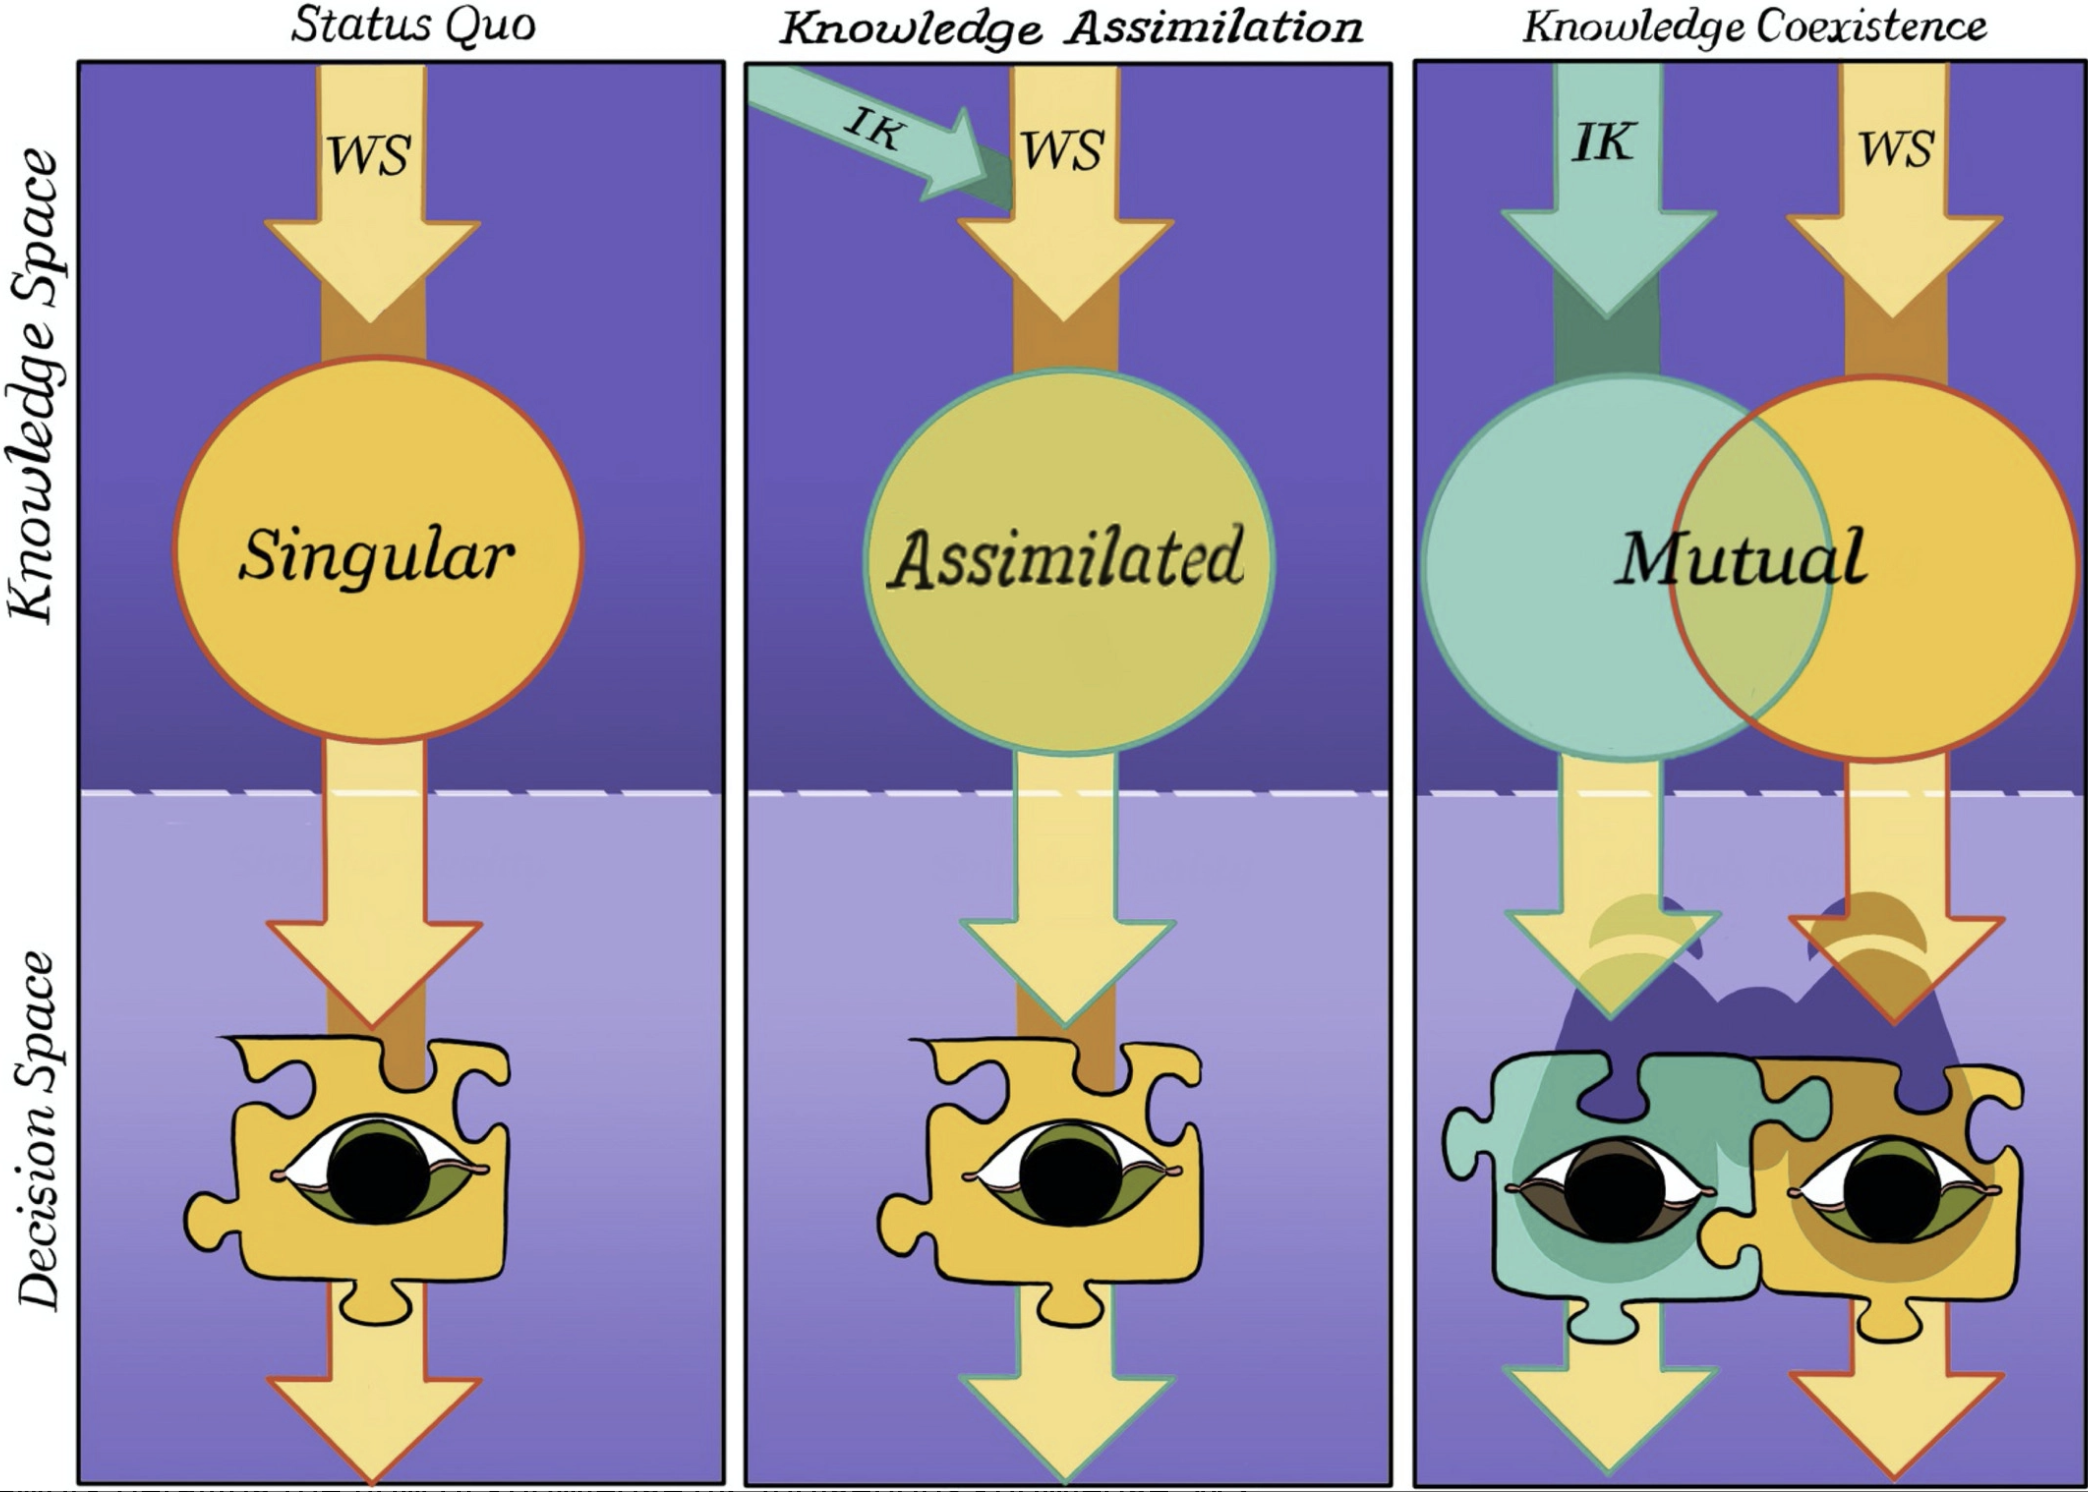
\includegraphics[width=29in]{images/Reid_2021} \caption{A conceptual framework detailing the flow of knowledge (Indigenous knowledge (IK); Western science (WS)) that underpins researchers’ understandings or views of reality, and ultimately guides their research and management decisions, as classified under three main archetypes. (Reid et al. 2021)}(\#fig:unnamed-chunk-10)
\end{figure}

\hypertarget{unsettling-marine-conservation-disrupting-manifest-destiny-based-conservation-practices-through-the-operationalization-of-indigenous-value-systems}{%
\subsubsection*{\texorpdfstring{``\href{(https://escholarship.org/uc/item/3sm1f1vq)}{Unsettling marine conservation: Disrupting manifest destiny-based conservation practices through the operationalization of Indigenous value systems}''}{``Unsettling marine conservation: Disrupting manifest destiny-based conservation practices through the operationalization of Indigenous value systems''}}\label{unsettling-marine-conservation-disrupting-manifest-destiny-based-conservation-practices-through-the-operationalization-of-indigenous-value-systems}}
\addcontentsline{toc}{subsubsection}{``\href{(https://escholarship.org/uc/item/3sm1f1vq)}{Unsettling marine conservation: Disrupting manifest destiny-based conservation practices through the operationalization of Indigenous value systems}''}

Lara A. Jacobs, et al.~\emph{Parks Stewardship Forum}. Vol. 38. No.~2. 2022.

Abstract exert: ``This paper is written by Indigenous scholars using Two-Eyed Seeing, reflexivity, and decolonizing methods (e.g., symbology, storytelling, and Indigenous beading) to unsettle the ways that marine conservation should be facilitated. Our framework operationalizes Indigenous value systems embedded within ``the seven R's'': respect, relevancy, reciprocity, responsibility, rights, reconciliation through redistribution, and relationships. This framework underlines the need for marine conservation efforts to center Indigenous voices and futures and Tribal management of marine systems. Marine system managers can use this paper as a guide for decolonizing marine conservation approaches, operationalizing Indigenous value systems in marine management, and building decolonial relationships with Indigenous Peoples and waters.''

\emph{If you are aware of other examples of Indigenous resource management, please share!}

Bryan, J. Walking the line: participatory mapping, Indigenous rights, and neoliberalism. Geoforum 42, 40--50 (2011). \url{https://www.sciencedirect.com/science/article/pii/S0016718510001090?via\%3Dihub}

Walter, M, Lovett, R, Bodkin Andrews, G and Lee, V. 2018. Indigenous Data Sovereignty Briefing Paper 1. Miaim nayri Wingara Data Sovereignty Group and the Australian Indigenous Governance Institute.

\end{document}
